%TODO In this document some things has to be relocated
\subsection{Product Perspective}
\subsubsection{User scenarios}
In this section are shown some scenarios in order to present some in real life settings and explain how CLup fits in and how it behaves in different situations.

% In this section some user scenario are shown in order to explain in real life settings how the CLup application works

\medskip

\textbf{Scenario 1: The Jet Market}

With the ``Stay home'' ordeal due to COVID-19 the ``Jet Market'', a mid sized grocery store in the city of Springfield experienced a sudden increase of customers per day. At the same time its not too big capacity was halved due to social distancing measures. These events lead to the formation of long queues of people out of the store premises in peak hours.

\smallskip

The store manager, in order to improve the service quality, decided to adopt the CLup queueing system. Upon signing the contract he received a business account, and set up the shop systems with the help of CLup advisors and technicians. In the very first days with CLup the queue length did not change much, but thanks to CLup adverts exposed outside the shop, some people downloaded the application.

\smallskip

In the following days more and more people noticing that CLup allowed to skip the line by booking the visit beforehand, downloaded the application too.

\smallskip

After some weeks the ``Jet Market'' can reserve up to the 60 \% of the store capacity to CLup booked customers. The remaining capacity is filled with non CLup customer. The ``Jet Market'' manager is very happy because the queues are a lot shorter and his customers started to distribute their visit more uniformly during the day.

\medskip

\textbf{Scenario 2: Bartolomeo}

Bartolomeo is an old grandfather. Due to his age he's not very familiar with the modern technology and he doesn't have a smartphone. His favorite supermarket decided recently to adopt CLup, as long queues were forming outside the store.

\smallskip

Before CLup adoption Bartolomeo waited up to one hour to enter the supermarket on peak times. After the installation, for customers not confident with the technologies used by CLup, like Bartolomeo, things did not become more complex. Bartolomeo has only to retrieve a paper ticket at the entrance and wait until his number is called. If there are a lot of people in queue before him, he could take a sit on the bench at the park near the supermarket and return in time for when his number is called. An estimation of the entrance hour is printed on every ticket.

\vfill


\textbf{Scenario 3: Slightly late}

Marcello booked the 5:45 PM slot at the supermarket near his workplace. This slot allows him to enter his chosen market from 5:45 PM to 6:00 PM without having to wait in line.

\smallskip

He normally ends his workday at 5:30 PM, but his colleague asked him some help just before him leaving. He arrived at the store late and scanned the ticket at 6:05 PM, just two minutes after the 3 minute tolerance (configured by the store using the CLup configuration panel).

\smallskip

The CLup system, considering that there are no people waiting in line and that the store is not full, lets Marcello enter anyway.
The application then sends him a notification reminding him that he could have possibily lost his priority, but saves him from the struggle of having to create an In-Site ticket and scan the code another time.

\medskip

\textbf{Scenario 4: Paperless}

For various reasons Adriana could not plan in advance when she could go grocery shopping at her favorite store this week.

\smallskip
On Thursday morning she was going to work by car, and received a call from her boss telling her that the scheduled meeting was cancelled. She had her morning free and decided to go for grocery shopping since she was already out of the house.

\smallskip

Even if she didn't book her entrance in advance, she used CLup to check how crowded the supermarket was. As she arrived near the supermarket, she created a ticket from the CLup application to enter as soon as possible. This kind of ticket is equivalent to the one printed by the emitter out of the store but it's paperless; moreover, the application notifies about live changes in the estimated entrance time. To avoid staying in front of the entrance Adriana waits in her car until CLup notifies her.
After some minute she recieves a notification on her phone that she should approach the entrance because in a short time she will enter the supermarket.

\medskip

\textbf{Scenario 5: No-show}

Luigi booked an entrance for the 4:00 - 4:15 PM slot last Saturday. He was busy cleaning the house and didn't pay attention to the time neither to his smartphone. At 4:30 PM he picks up the phone and notices CLup notifications about approaching the entrance, and even about that his picked timeslot to enter had expired.

\smallskip

Since he forgot to cancel his booking, at 4:20 PM the late tolerance time ended. The store at the time is unusually full and some people are waiting outside. CLup system allowed one more person to enter the store replacing Luigi's reservation.

\vfill



\subsubsection{The world and the machine}
In this section the system will be described using ``The World and The Machine'' model proposed by M. Jackson.
At a coarse grain CLup is composed from a central system (the machine) which relates with some components that allow shared phenomena to happen between the world and the machine happen

\begin{figure}[H]
    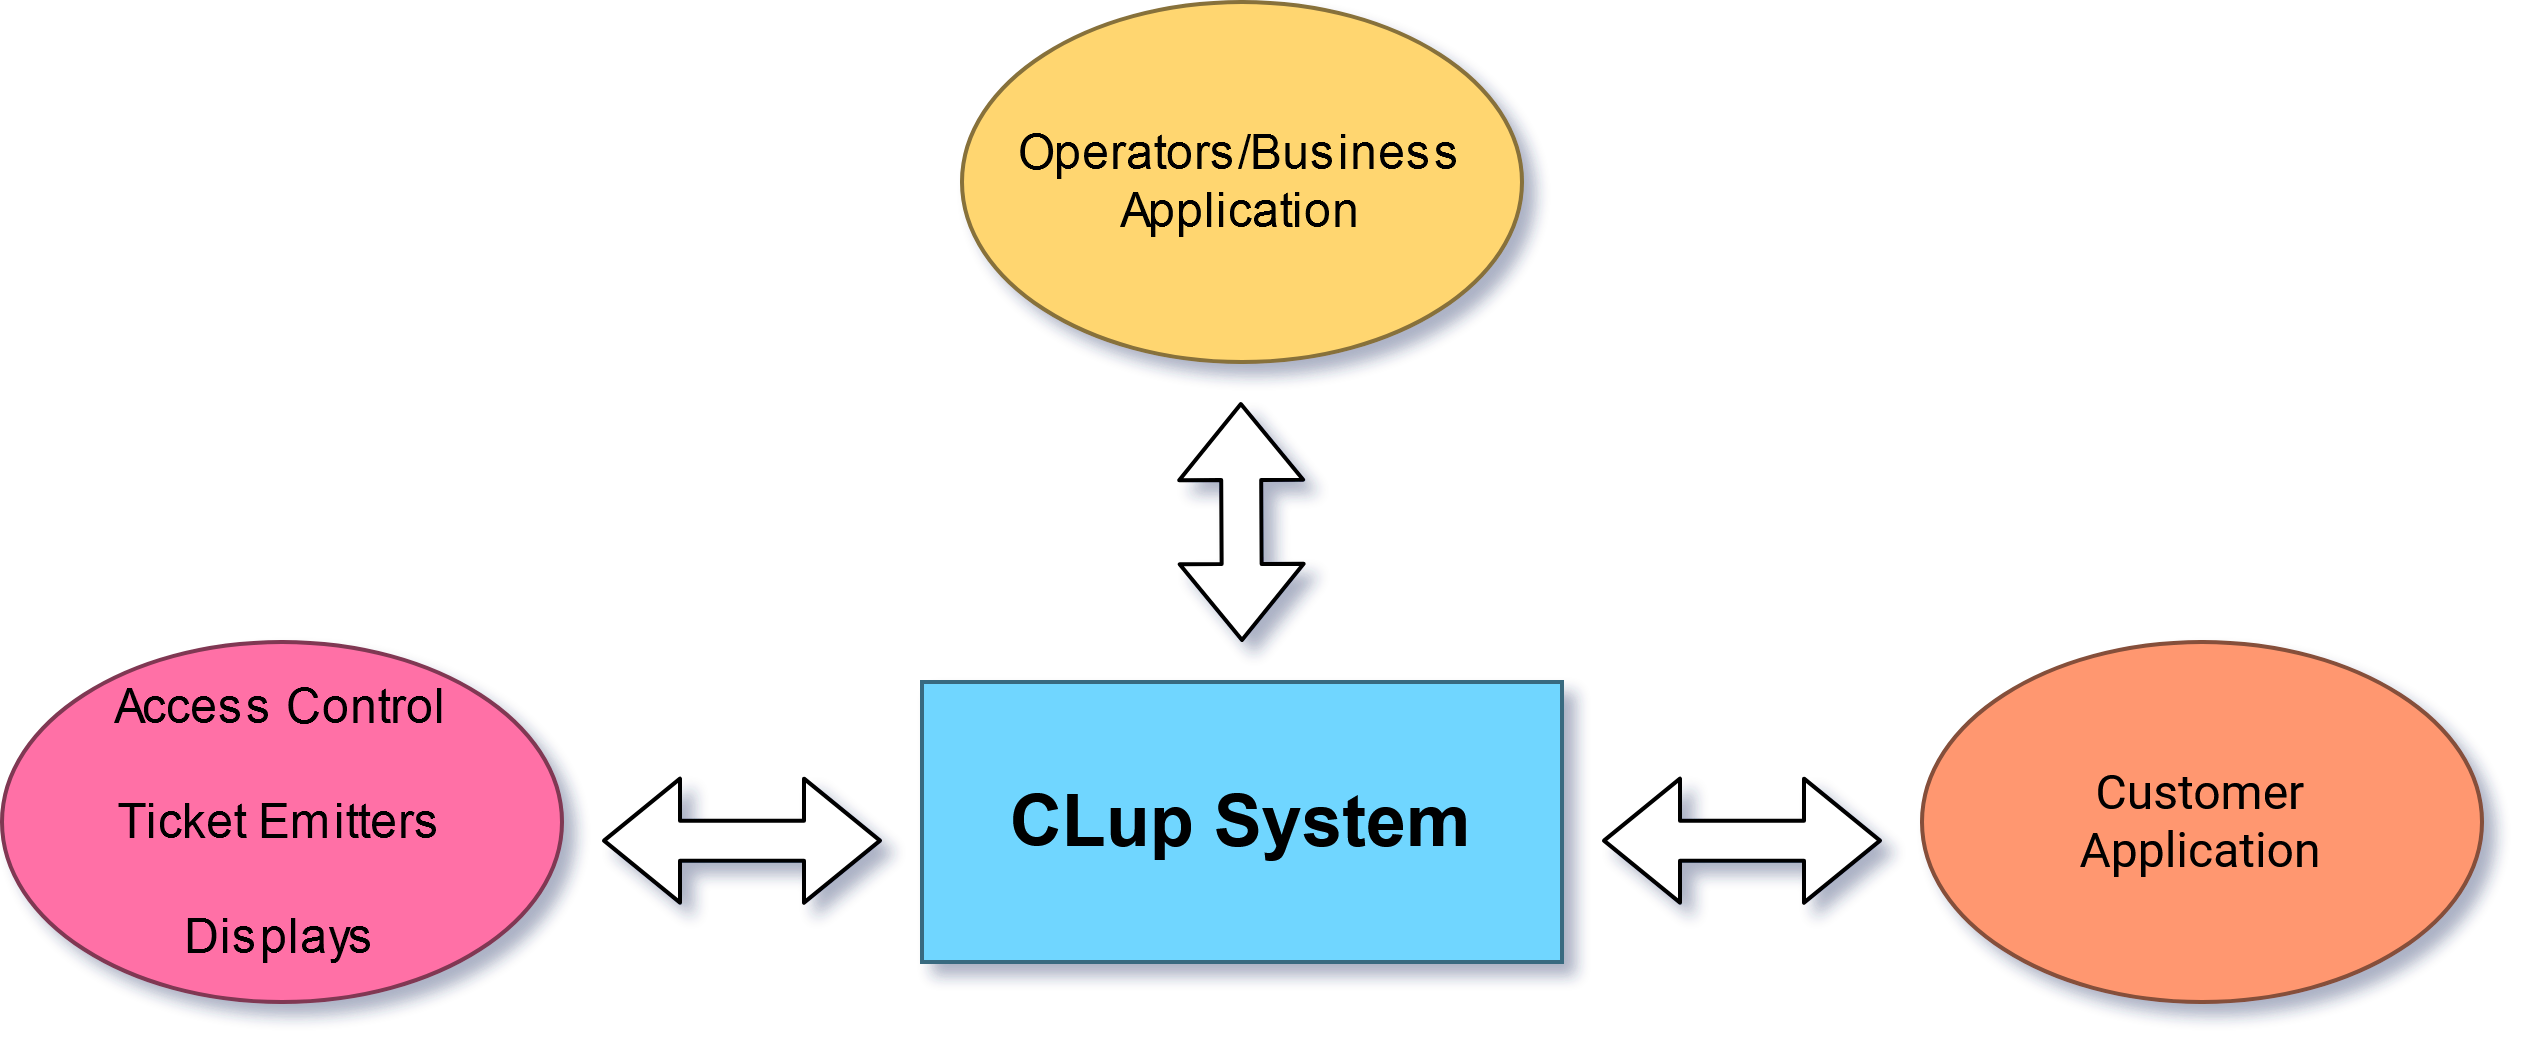
\includegraphics[width=\textwidth]{Images/system2.png}
    \caption{\label{fig:Coarse_Grain_System}``The Machine'' and the components interfacing with ``The world''}
\end{figure}

\subsubsection{Shared phenomena}
%TODO: Probably to be relocated
Here is a list of shared phenomena happening in CLup

\rowcolors{2}{gray!25}{white}
\renewcommand{\arraystretch}{1.4}
\begin{tabular}{C{1cm}L{10.5cm}C{2.6cm}}
    \rowcolor{gray!50}
    Label & Phenomena                                                                                                  & Controlled by \\
    SP1   & The gate opens and lets the customer inside the store                                                      & Machine       \\
    SP2   & The customer scans his ticket at the gate                                                                  & World         \\
    SP3   & The customer leaves the store and their exit is counted by a People-Counting System                        & World         \\
    SP4   & The customer books a ticket to enter the shop with the Customer Application                                & World         \\
    SP5   & The customer receive a notification when his almost his turn to enter the store                            & Machine       \\
    SP6   & The customer presses the button to request a paper ticket                                                  & World         \\
    SP7   & The customer receives a ticket from the ticket printer and an estimated waiting time                       & Machine       \\
    SP8   & The display at the entrance shows which ticket numbers are allowed to enter and the other numbers in queue & Machine       \\
\end{tabular}

\subsubsection{Interfacing with external systems}
The S2B will expose some interfaces to communicate with external systems used to provide data to CLup.


\textbf{Physical ticket emitters} should be placed outside the store near the entrance, to allow users that do not have CLup installed on their smartphones to wait for their entrance. The ticket emitter prints tickets on a paper support when a button is pressed. The emitter has an internet connection and via a dedicated API request retrieves information for a new valid ticket. The response will contain the needed information to print the ticket (e.g. the ticket number/QR code and the estimated time before entering). The queue statistics in the system are then updated accordingly.

Optionally the emitter could have a small screen to show the current waiting time estimation, so customers can know in advance if they have the possibility to wait for the displayed time.


A \textbf{Smart gate} is a composed of a mechanical actuator that opens and closes the gate, a QR code scanner and it is provided with internet connectivity. When a QR code is scanned and decoded, a request is sent to the CLup API with the ticket information stored in the code.
The system checks the validity of the ticket and sends a response to the gate. If the response is affirmative the gate will open, if the scanned QR doesn't represent a valid ticket an error will be shown to the customer via visual and/or auditive feedbacks. Even if the gate replaces a big part of access-control staff's work (see next paragraph), some human intervention could be required for security reasons, or to open the gate in exceptional cases.


\textbf{People counters} located at shop exits count people passing through that exit. They are connected to the network and will communicate the count of people that left the shop. This counter could be a turnstile or a sensor; it could even be another smart gate that scans the same tickets used to enter (or a barcode printed on the receipt) before letting people out of the store.

CLup system should works fine without them, but these counter allow to have a precise count of the people inside the shop, and this datum could be useful to estimate more precisely the waiting times. In particular, CLup can calculate and store the shopping time of customers if it's given the possibility to associate the time of entrance with the time of leaving of the said customer. This could, for example, be done through the scan of the same QR code for both entering and leaving.


\textbf{Ticket number screens} are located at shop entrances. They display the latest batch of ticket numbers allowed to enter the store, and the ordered list of the other numbers in line.

\vfill


\subsubsection{Interfacing with users}

\textbf{Access-control operators} have a portable device equipped with a camera and internet connectivity. This device has installed the staff access-control app. The user interface for operators provides these functionalities:
\begin{itemize}
    \item Authenticate with a CLup operator account or corporation SSO service
    \item Check (and adjust) estimated occupancy of the whole shop and its departments
    \item Check length of the queues, and bookings in the time slots
    \item Scan a ticket QR code to manually allow a person to enter
    \item Notify the next customers in the virtual ticket queue alerting them to reach the entrance
\end{itemize}

The \textbf{CLup Customer Application} allows some operations even to unauthenticated users, though only logged in ones can book tickets for In-Site queues or for a desired time slot.
\begin{itemize}
    \item Every user can:
          \begin{itemize}
              \item Create a new account
              \item Login to an existing account
              \item Check which nearby stores are adopting CLup system (on a map) and an option for listing them sorted by distance
              \item See real-time and projected occupancy of all stores
          \end{itemize}
    \item An authenticated user can also:
          \begin{itemize}
              \item Create a virtual ticket to enter a store immediately (if space is available) or join a queue and get update notifications
              \item Check store occupancy in future time slots
              \item Book a visit to a selected store in an available time slot
          \end{itemize}
\end{itemize}

\vfill
\pagebreak

\subsection{User Characteristics}
There are two macro-groups of people that will use CLup, the businesses adopting the system and the customers of these
business using CLup to plan their visits to the shop.
\subsubsection{Business-side Characteristics}
CLup is addressed mainly to big grocery shops, but could be used from every medium to big sized shop.
CLup is very flexible, and will work adapting to a lot of different scenarios, thanks to these features:
\begin{itemize}
    \item Parameters of the system are tunable: The business is able to customize booking time-slots duration and capacity
    \item Different access controls methods can be employed: The shop could install smart gates with a QR scanner or could delegate an employee to manually check the tickets with a the CLup business mobile application.
    \item Different precision levels of estimated data are accessible based on the data sources available. For example, if the shop counts the number of people exiting the premises (using a turnstile or a QR scanner), CLup can provide the exact live occupancy of the store. If this is not possible, the live occupancy will be estimated based on the average permanence time in the shop.

\end{itemize}
\subsubsection{Customer side characteristics}
Everyone needs to do grocery shopping, but in the situation of a pandemic, it is encouraged to stay safe at home. This can lead people to go for longer shopping sessions to last more days without going out; it can also drastically increase the number of customers per day at supermarkets, inevitably creating long queues.
Nobody should be excluded from accessing the shops, and also people without CLup application need to be taken into account.


The S2B solves this problem by allowing those customers to retrieve paper tickets and wait in a physical line before entering the shop if the shop is full.
The physical line of customer is unavoidable if the supermarket cannot satisfy the increased demand of groceries in its area, even if CLup can alleviate this problem allowing a better distribution of the client visits.The possibility of booking visits in advance will push more and more users to download CLup in ordert to avoid queues; avoiding cramming at the entrance and maintaining social distancing can decrease the spread of the virus.

\vfill

\subsection{Assumptions and dependencies}
\subsubsection{Domain Assumptions}

\rowcolors{2}{gray!25}{white}
\renewcommand{\arraystretch}{1.4}
\begin{tabular}{C{1cm}L{14.1cm}}
    \rowcolor{gray!50}
    Label & Domain Assumption                                                                                                                                                                                  \\

    DA1   & Customers that created a shoplist will buy approximately all the products in that list, so they will visit for the greater part of their permanence the departments where the products are located \\

    DA2   & Customer will stay approximately the time they have declared when booking the ticket                                                                                                               \\

    DA3   & The access-control system works properly and won't allow unauthorized customer entrances                                                                                                           \\

    DA4   & Customers with an in-place digital ticket try to avoid staying near the entrance until they receive the ``go to entrance'' notification                                                            \\

    DA5   & Customers with a booked ticket in a given time slot will not show up until few minutes before the start of their time slots                                                                        \\

    DA6   & If people-counters are installed they will provide the exact count of the customers that enter or leave the shop                                                                                   \\

    DA7   & No customer are present at the shop opening hour, and no customer will be present at the shop closing hour                                                                                         \\

    DA8   & The store manager will insert correct data about the shop and the departments maximum capacities                                                                                                   \\
\end{tabular}

% \subsubsection{Dependencies}
% \subsubsection{Constraints}

\vfill
\pagebreak

\subsection{Product Functions}

In this section are presented the main functions of the S2B, introduced by the state machines representing the two main scenarios for the customers.

\begin{figure}[H]
    \centering
    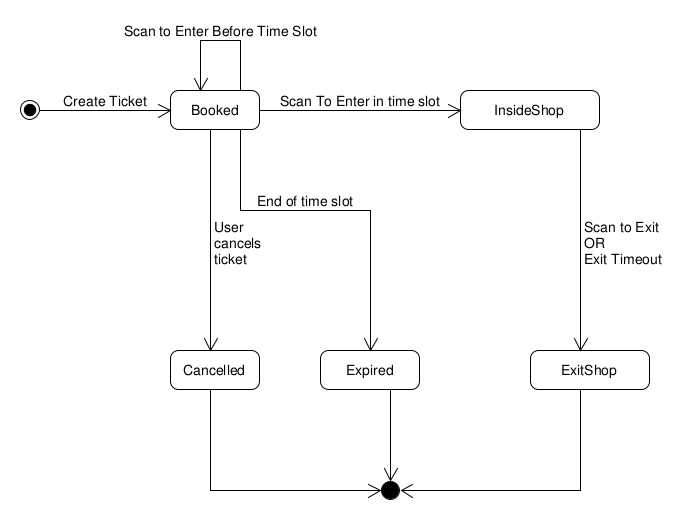
\includegraphics[width=\textwidth]{Images/UML_booked_ticket.png}
    \caption{\label{fig:Booked_Ticket_State}Booked ticket state machine}
\end{figure}

\vfill
\pagebreak

\begin{figure}[H]
    \centering
    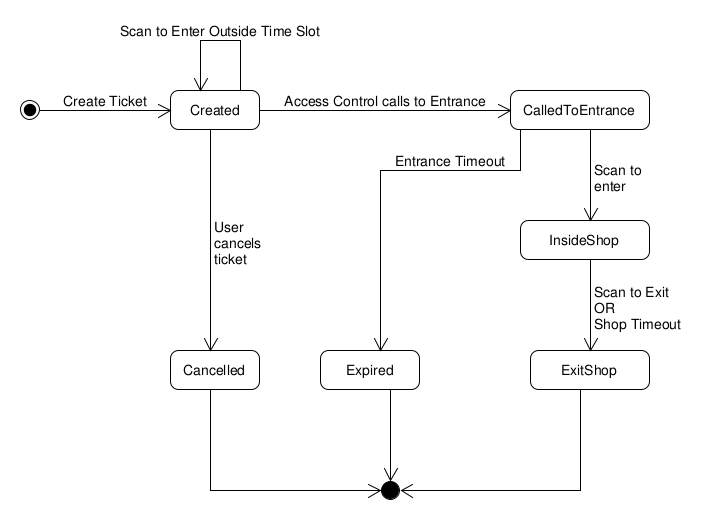
\includegraphics[width=\textwidth]{Images/UML_in_place_virtual_ticket.png}
    \caption{ \label{fig:Booked_Ticket_State}In-place virtual ticket state machine}
\end{figure}

Keeping in mind this two state machines it is provided a list of requirements for the CLup system.
Every interaction should be taken into account and implemented in the most simple and user friendly way.
The effort put into realizing the best user experience should be priorized towards the customers that will use the application. Stores adopting the CLup system should instruct their workers on how to use the application; customers should receive the most immediate and intuitive UX as possible.

Requirements list both functional and non-functional requirements, and span every aspect the system will have to implement and respect to achieve all the previously described goals. Further in the document, goals will be mapped with the requirements needed to fullfil them, to provide a convenient reference useful to understand how much work will be needed to accomplish goals and how to divide teams for development.

\vfill

\subsubsection{System Requirements}

\rowcolors{2}{gray!25}{white}
\renewcommand{\arraystretch}{1.4}
\begin{tabular}{C{1cm}L{14.1cm}}
    \rowcolor{gray!50}
    Label & Requirement description                                                                                                                                                                     \\

    R11   & The system must keep general information and contacts about the store chains adopting CLup                                                                                                  \\
    R12   & The system must provide each store a store-admin account                                                                                                                                    \\
    R13   & The store-admin account must allow the creation of store-operator accounts                                                                                                                  \\
    R14   & For each store the system must allow the users to retrieve information about location and business hours                                                                                    \\
    R15   & The system stores information about capacity of each market                                                                                                                                 \\
    R16   & The system won't let anyone enter the store if the maximum capacity has been reached                                                                                                        \\
    R17   & The system will let a customer enter the store if and only if he has a a valid ticket                                                                                                       \\
    R18   & The system will use the occupancy data retrieved from the supermarket to control the store access                                                                                           \\
    R19   & The system must provide an interface for communicating with the store access control                                                                                                        \\
    R21   & The system must provide an interface for user to compile a shopping list                                                                                                                    \\
    R22   & The system must take in consideration shopping list data and historic data from previous user visits to reduce store crowdedness per department                                             \\
    R31   & The system must allow the store-admin account to create and edit entrance time intervals                                                                                                    \\
    R32   & Each time interval must have a number of bookable slots fewer than the store capacity                                                                                                       \\
    R33   & The system must allow authenticated users to book a visit in a desired time interval                                                                                                        \\
    R34   & The system must not allow a user to book a slot in an already full time interval                                                                                                            \\
    R35   & The system must not allow a user to book a visit if he has already reserved another visit                                                                                                   \\
    R36   & The system must allow a customer to create a numbered virtual queue ticket and notify them if he can enter immediately (if the store is not full) or provide them a waiting time estimation \\
    R37   & The system must notify the customers with a virtual queue ticket when it's time to approach the store entrance                                                                              \\
    R38   & The store operator application must allow an authenticated operator to manually admit customers                                                                                             \\
\end{tabular}

\vfill

\begin{tabular}{C{1cm}L{14.1cm}}
    \rowcolor{gray!50}
    Label & Requirement description                                                                                                                                                         \\
    R42   & The system  must ask the customer to provide the estimated visit time when booking a time slot                                                                                  \\
    R51   & The system must allow stores to hand out numbered physical queueing tickets to those that do not use the CLup application                                                       \\
    R52   & The system must allow the access to the store to customer with numbered tickets using a First Come First Served logic, treating virtual and physical ticket owner equally       \\
    R53   & The system must try to estimate waiting time based on store capacity, reservations and the current number of people with numbered tickets waiting in line                       \\
    R54   & The system should interface with an screen placed at the entrance of the store to notify customer which ticket number enters next                                               \\
    R61   & The system must let the store-admin accounts retrieve statistics collected from CLup regarding their store                                                                      \\
    R62   & The system must record periodically and store statistics about the occupancy of each store                                                                                      \\
    R63   & The customer CLup application must show brief statistics about average occupancy of each stores during different days of the week                                               \\
    R64   & The operator CLup application must show to an authenticated operator the real time occupancy of the store                                                                       \\
    R71   & The customer CLup application must be cross-platform and must work on the majority of the devices                                                                               \\
    R72   & The stores adopting CLup must be displayed on a map                                                                                                                             \\
    R73   & The CLup customer application allows user to mark stores as favorite in order to access them quickly                                                                            \\
    R74   & The CLup customer app after the login allows immediately to book tickets right from the homepage                                                                                \\
    R81   & The system must provide an interface for automated control devices to communicate to CLup data about store entrances, store leavings and crowdedness in the various departments \\
    R91   & The system must push notifications to user devices with update information on the store he has a ticket for                                                                     \\
    R101  & The system must associates tickets with line numbers                                                                                                                            \\
\end{tabular}
\vfill

\subsubsection{System Representation}

Use cases and scenarios, elaborated and expanded into functional and non-functional requirements for the software, require a structure defining all the entities involved in the system.
Below it is presented the CLup class diagram, with interaction between entities and the cardinality of such associations.

\begin{figure}[H]
    \centering
    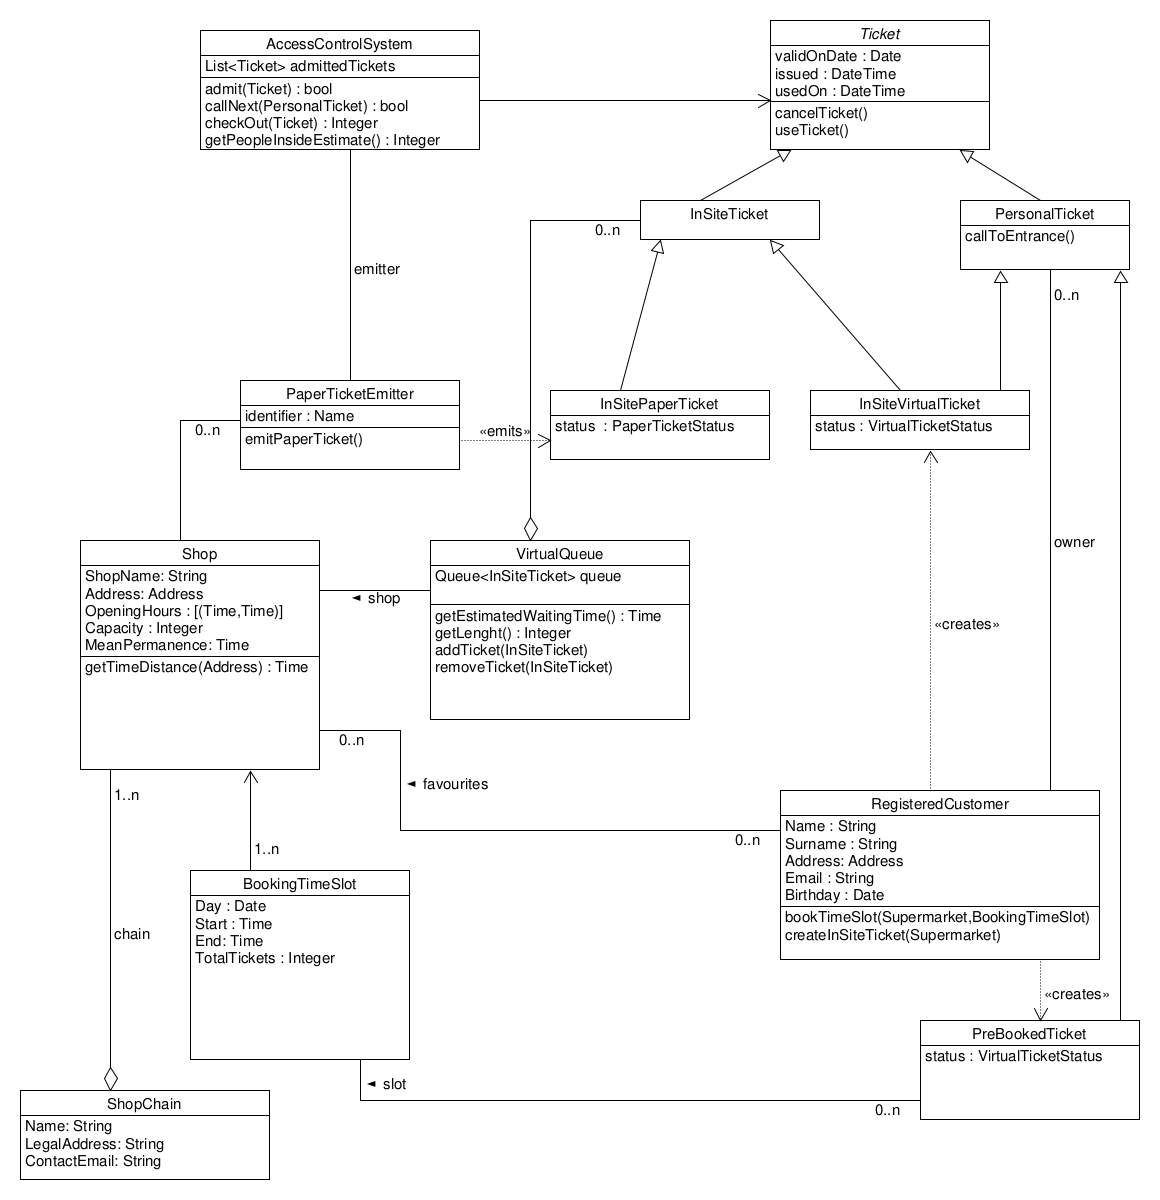
\includegraphics[width=\textwidth]{Images/UML_class_synthetic.png}
    \caption{\label{fig:Booked_Ticket_State}Class Diagram}
\end{figure}

\vfill
